% This is a spreadsheet containing the generic names of the player and
% antagonistic elements and their game properties. 

% This should allow an easy cross reference for an elements in the game
% that a value. 
\subsection{Spillmatrisen}
Spillmatrisen (se Figur~\cite{fig:spillmatrise}) er en grafisk forklaring
på hvilke elementer i spillet som interagerer med hverandre. Elementer
som våpen, forsvar og oppgraderinger er kun beskrevet på et overordnet
nivå, siden disse elementene deler like egenskaper (f.eks. at alle
angrep kan angripe forsvar).
\begin{center}
\begin{figure} [H]
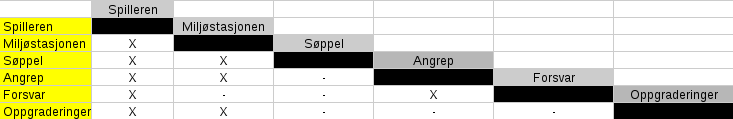
\includegraphics[scale=0.6]{images/spillmatrise.png}
\label{fig:spillmatrise}
\caption{Spillmatrise med de forskjellige elementene}
\end{figure}
\end{center}
I Figur~\cite{fig:spillmatrise} er elementene som interagerer er merket
med en \textbf{X} i den kollonnen og raden de elementene sammenfaller i.
Hvordan elementene interagerer er beskrevet nedenfor:
\begin{description}
\item \textbf{Spilleren}\\Spilleren sin oppgave er å samle søppel,
bygge våpen og forsvar, samt oppgradere miljøstasjonen.
\item \textbf{Miljøstasjonen}\\Miljøstasjonen tar imot og gjenvinner
søppelet. I tillegg er dette hovedbasen for spilleren, og står for alle
oppgraderingene. En miljøstasjon kan bli angrepet av andre spillere, og
interagerer derfor med våpen.
\item \textbf{Søppel}\\Blir plukket opp av spilleren, og lagt på
miljøstasjonen for gjenvinning.
\item \textbf{Angrep}\\Spillere kan angripe andre spillere sitt forsvar,
og miljøstasjonene deres.
\item \textbf{Forsvar}\\Forsvaret kan bli angrepet og ødelagt av våpen.
En spiller bygger forsvaret, derfor koblingen mellom spiller og forsvar.
\item \textbf{Oppgraderinger}\\Spilleren kan oppgradere miljøstasjonen
sin. Desse oppgraderingene baserer seg på statusen til miljøstasjonen.
\end{description}

